\documentclass[12pt,twoside,onecolumn]{article}

\usepackage{a4}
\usepackage[dvipsnames]{xcolor}
\usepackage[margin=0.75in]{geometry}
\usepackage{pdfpages}
\usepackage{apacite}
\usepackage{jneurosci}
\usepackage[utf8]{inputenc}
\usepackage[T1]{fontenc}
\usepackage[norsk]{babel}
\usepackage{subfiles} % Handeling multiple chapters on seperate files.
\usepackage{graphicx}  % for displaying figures
\usepackage{subcaption}
\usepackage{url}
\usepackage{amsmath} % math package
\usepackage{relsize} % to use larger math symbols
\usepackage{amssymb} % for using blackboard letters (e.g R for real numbers)
\usepackage{tocbibind} % for adding the reference section in table of contents
%\usepackage{fixltx2e} % for text in sub script
\usepackage{perpage} % for resetting footnote counter at each page
\usepackage{csquotes}
\usepackage{epigraph}
\usepackage{ragged2e}

\MakePerPage{footnote} %the perpage package command

\addto\captionsenglish{%
  \renewcommand{\figurename}{Figur}
}

\makeatletter
\def\@documentnocite#1{\@bsphack
  \@for\@citeb:=#1\do{%
    \edef\@citeb{\expandafter\@firstofone\@citeb}%
    \if@filesw\immediate\write\@auxout{\string\citation{\@citeb}}\fi
    \@ifundefined{b@\@citeb}{\G@refundefinedtrue
      \@latex@warning{Citation `\@citeb' undefined}}{}}%
  \@esphack}
\AtBeginDocument{\let\nocite\@documentnocite}
\makeatother

\begin{document}

Denne skriften er det brukeren ser\newline
{\color{gray} Skriften brukes til å refere til manus} \newline
{\color{PineGreen} Skriften brukes til å refere til videodesigner} \newline
{\color{Maroon} Skriften brukes til å refere til handlinger i plattformen}
\section*{Ligninger}

\subsection*{Førstegradsligninger}

\textbf{Oppgave 1}
\begin{align}
7x - 3 &= 11  \qquad\text{ Plus 3 på begge sider av likhetstegnet.}\\
7x -3 +3 &= 11 + 3\\
7x &= 14\\  
\frac{7x}{7} &=  \frac{14}{7} \qquad\text{ Uttrykket kan forkenkles mer.}\\
x &= 2
\end{align}
\newline
\textbf{Oppgave 2}
\begin{align}
\frac{x}{2} + \frac{5}{6} &=  \frac{4}{3} - x \qquad\text{ Pluss x på begge sider av likhetstegnet.}\\
\frac{x}{2} + x + \frac{5}{6} &=  \frac{4}{3} - x + x\\
\frac{x}{2} + x + \frac{5}{6} - \frac{5}{6} &=  \frac{4}{3} - \frac{5}{6}\\
\frac{x}{2} + \frac{2x}{2} &= \frac{8}{6} - \frac{5}{6}\\
\frac{3x}{2}  &= \frac{3}{6} \qquad\text{ Uttrykket kan forkenkles mer.}\\ 
\frac{3x\cdot2}{7\cdot3} &=  \frac{1\cdot2}{2\cdot3} \qquad\text{ Uttrykket kan forkenkles mer.}\\
x &= \frac{1}{2}
\end{align}

\subsection*{Sett inn tall i formler}
\textbf{Oppgave 3}
Fatima har kjøpt nytt abonnement hos Telihor. I abonnementet har hun en fast beløp hver måned på 50 kr. I tillegg må hun betale 1.50 kr per MB hun bruker. 
\newline\newline
\textbf{Del 1)} Lag en ligning som beskriver Fatimas total månedlig kostnad. La x være antall MB hun bruker i måneden og P(x) hennes total kostnad per måned.
\begin{align}
P &= 50 \text{ Hvis Fatima bruker ingen data, blir da hennes forbruk lik 50}\\ 
P &= 50 + 1.5\cdot1\text{ Hvis Fatima bruker 1MB data, blir da hennes forbruk lik $50 + 1.5\cdot1$}\\ 
P &= 50 + 1.5\cdot2\text{ Hvis Fatima bruker 2MB data, blir da hennes forbruk lik $50 + 1.5\cdot2$}\\ 
&\text{ Hva blir hennes forbruk hvis hun bruker x-antall data per måned} \nonumber\\
P &= 50 + 1.5x
\end{align}
\newline
\textbf{Del 2)}
Finn hennes total kostnad per måned når hun bruker 1000 MB = 1 GB data.
\begin{align}
P &= 50 + 1.5\cdot1000\\
P &= 50 + 1500\\
P &= 1550
\end{align}
Vil du si at dette er et bra abonnement for Fatima i år 2017 ?

\section*{Funksjoner}

\subsection*{Stigningstallet}
\textbf{Oppgave 1}
Vennligst klikk følgende koordinat i planet:$(0,1)$
\begin{figure}[h!]
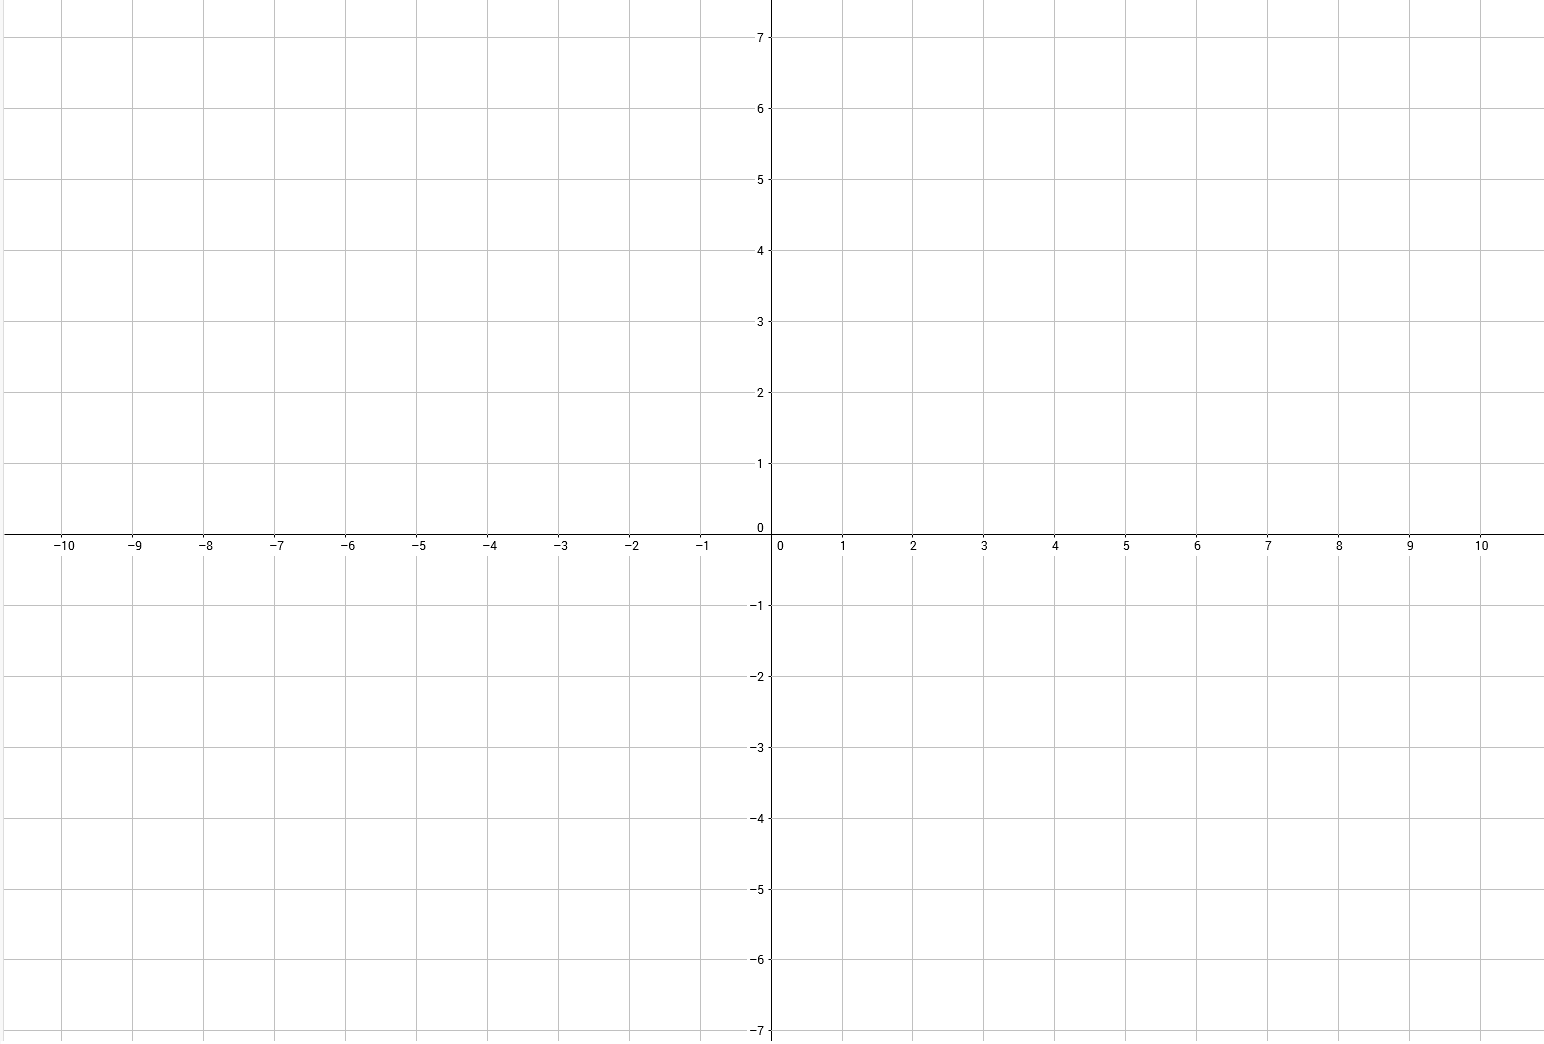
\includegraphics[scale = 0.3]{figures/Grid.png}
\label{fig:grid}
\end{figure}
\newline
{\color{Maroon}Hvis bruker taster feil, får han lov til en ny sjanse}
\newline
Vennligst klikk følgende koordinat i planet: $(3,1)$
\newline
{\color{Maroon}Hvis bruker taster feil denne gangen vil han få en hint - hint knappen blir synlig}
\newline\newline
\textbf{Hint:}  $(x,y) = (3,1)$, dvs. at $x = 3$ og $y = 1$. Prøv å vis dette punktet i planet.
\newline
\newline
{\color{Maroon}Hvis bruker taster feil på flere slike oppgaver vil han få en video med forklaring :} 
\newline
La oss se på punkt (4,2) og (-3,5). Vi vil nå vise at disse punktene ligger henholdsvis i første og andre kvadrant.
Husk at den horisontale koordinat aksen (x-aksen) er alltid den første koordinat ({\color{PineGreen}På videoen blir et punktene hevet med grafikk}), mens det andre tallet i tall paret er langs den vertikale koordinat aksen (y-aksen).
\newline
\newline
{\color{Maroon}Hvis bruker taster riktig på flere slike oppgaver vil han gå videre til neste oppgave.}
\newline\newline
\textbf{Oppgave 2} \newline
Finn stignigstallet til følgende lineær funksjoner. Fyll svaret i svarfeltet :
\begin{figure}[h!]
\centering
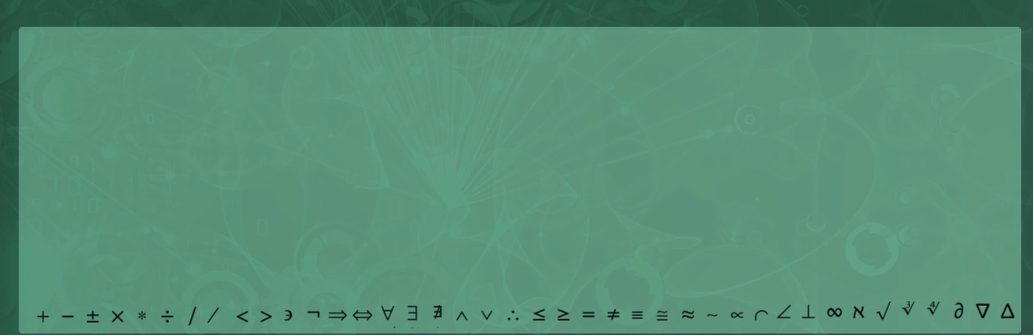
\includegraphics[scale = 0.3]{figures/Svarfelt.png}
\label{fig:grid}
\end{figure}
{\color{Maroon}Hvis eleven taster feil:} Husk at stigningstallet beskriver hvor mye funksjonen vokser eller minker når du øker x verdien. Husk at stigningstallet er gitt som forandring i y-verdien delt på forandringen i x-verdien:
\begin{align}
a = \frac{\Delta y}{\Delta x} = \frac{y_2 - y_1}{x_2 - x_1}
\end{align}
\begin{figure}[h!]
\centering
    \begin{subfigure}{.5\textwidth}
    \centering
    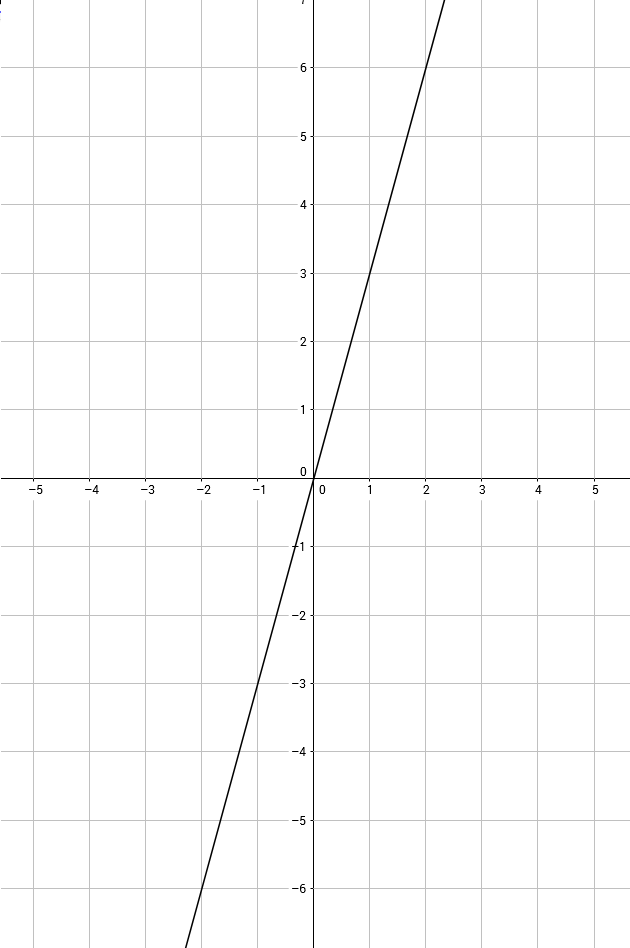
\includegraphics[scale = 0.5]{figures/3X.png}
    \end{subfigure}%%
    \begin{subfigure}{.5\textwidth}
    \centering
    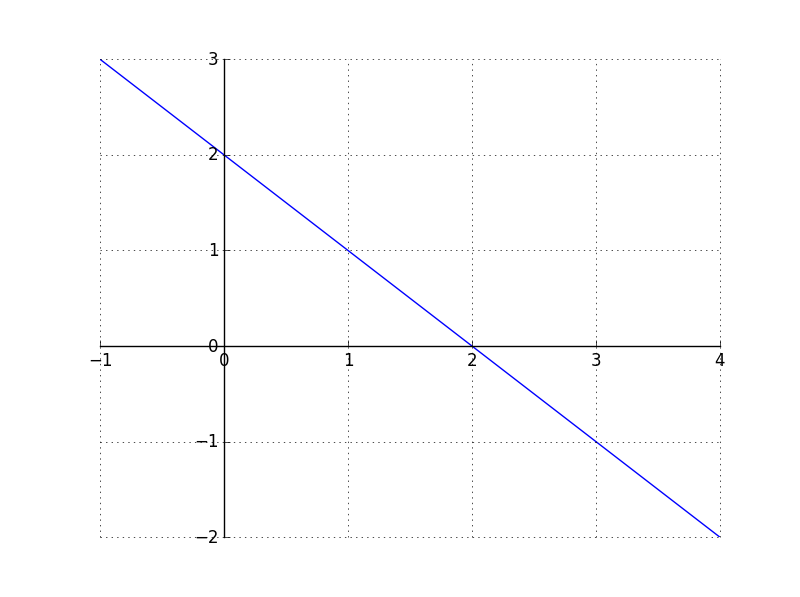
\includegraphics[scale = 0.5]{figures/mXp2.png}
    \end{subfigure}
    \begin{subfigure}{.5\textwidth}
    \centering
    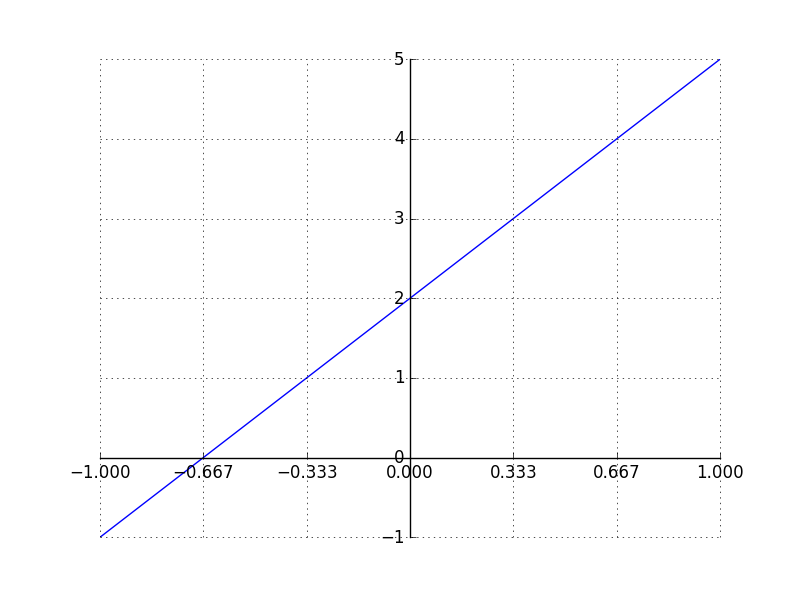
\includegraphics[scale = 0.5]{figures/3Xp2.png}
    \end{subfigure}%%
    \begin{subfigure}{.5\textwidth}
    \centering
    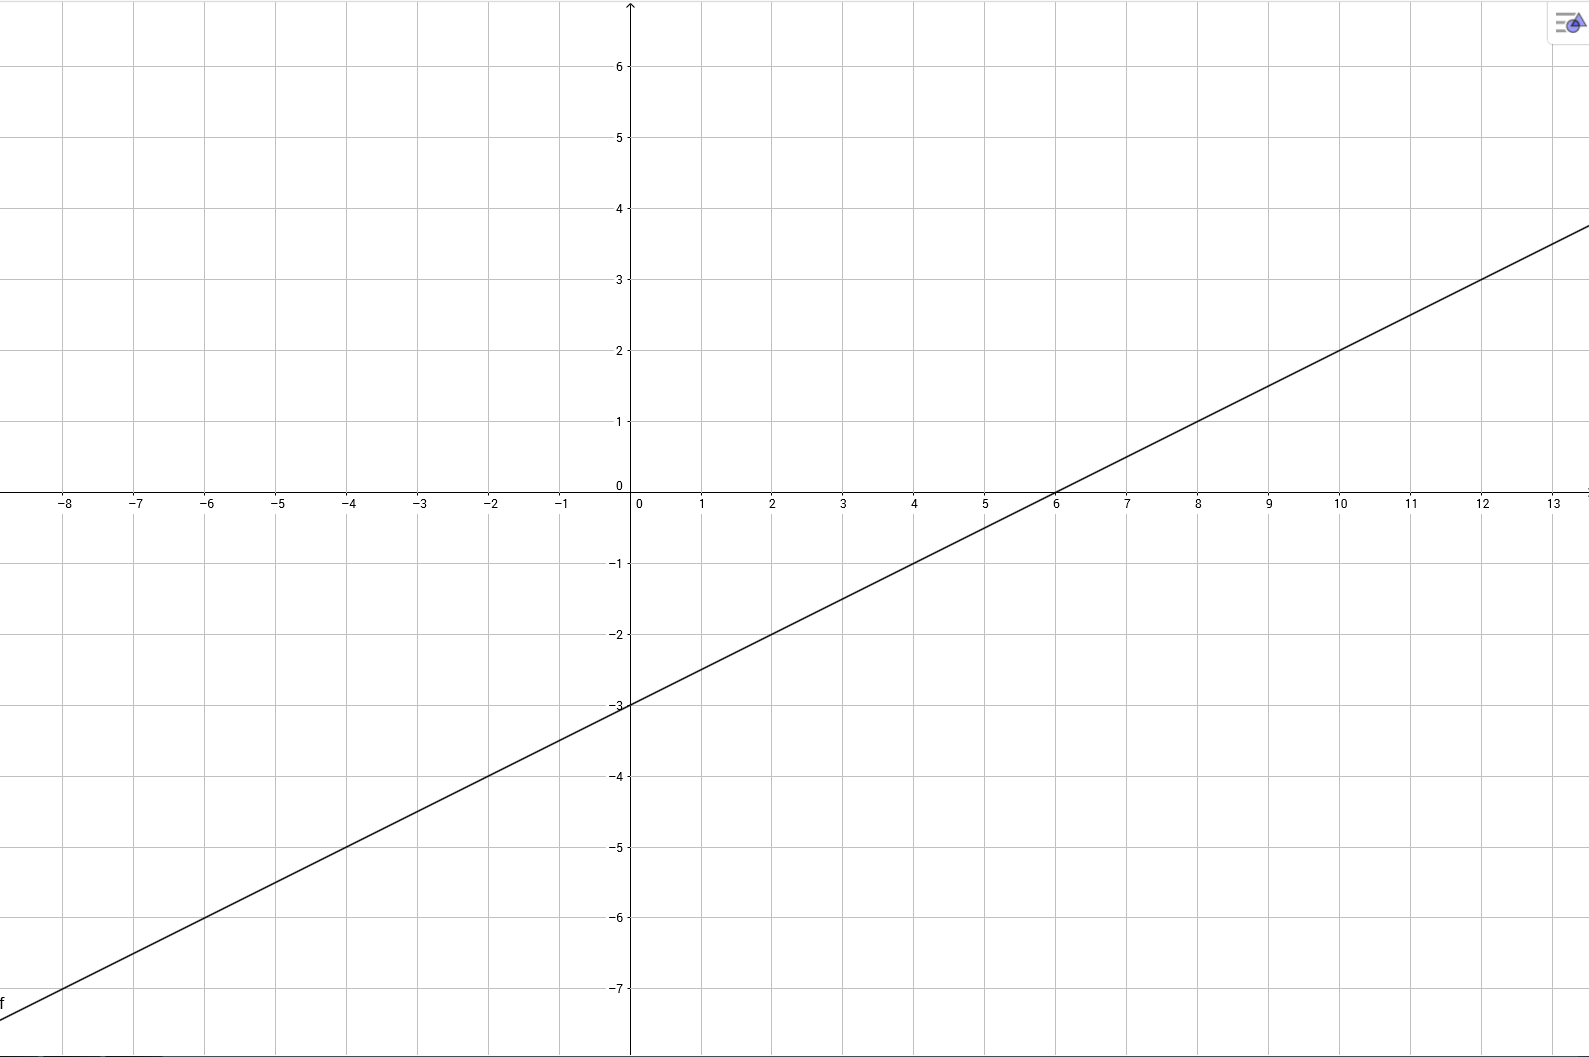
\includegraphics[scale = 0.5]{figures/05Xp2.png}
    \end{subfigure}
\end{figure}
{\color{Maroon}Hvis eleven forsatt ikke forstår vil da eleven presenteres med en video forklaring :  Video forklaring knappen dukker opp.}
\newline
\newline
\textbf{Video forklaring:}
\newline\newline
{\emph{\color{gray}
Husk at stigningstallet kan regnes ved å dele forandringen mellom y verdiene på forandringen i x-verdiene.}} 
\newline
{\color{PineGreen} På videoen vises formelen mens det forklares vha. grafen hvor oppleseren trekker en vertikal linje ned fra grafen fra en passelig funksonsverdi og deretter trekkes det en linje horisontalt inntil til funksjonen.} \newline\newline
{\emph{\color{gray}
Jeg kan velge passende $\Delta y$ og $\Delta x$ verdiene og sette disse inn i formelen for å regne ut stigningstallet.}} \newline
{\color{PineGreen} Det vises at oppleseren markerer $\Delta y$ og $\Delta x$ på grafen og skriver opp formelen.} 
\begin{figure}[h!]
\centering
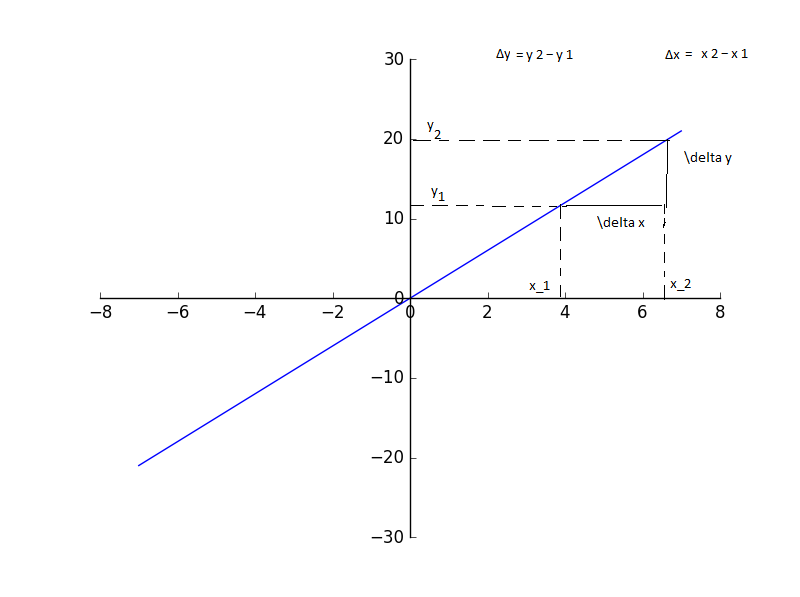
\includegraphics[scale = 0.4]{figures/stigningstallet.png}
\end{figure}
\newline\newline
{\emph{\color{gray}
F.eks i funksjonen $y = 3x$. Vi velger disse to punktene $y_2$ og $y_1$. Her ser vi at forandringen i y, er $\Delta y = y_2 - y_1 = 6- 0$ og forandringen i for disse funksjonsverdiene er $\Delta x_2 - \Delta x_1 = 2 - 0$. Da ser vi at stigningstallet blir $6/2 = 3.$}} \newline
{\color{PineGreen} Det vises at oppleseren gjentar avlesning fra funksjonen og markerer verdiene med striplet linje. Deretter setter oppleseren verdiene inn i formelen og regner ut stigningstallet.}
\begin{figure}[h!]
\centering
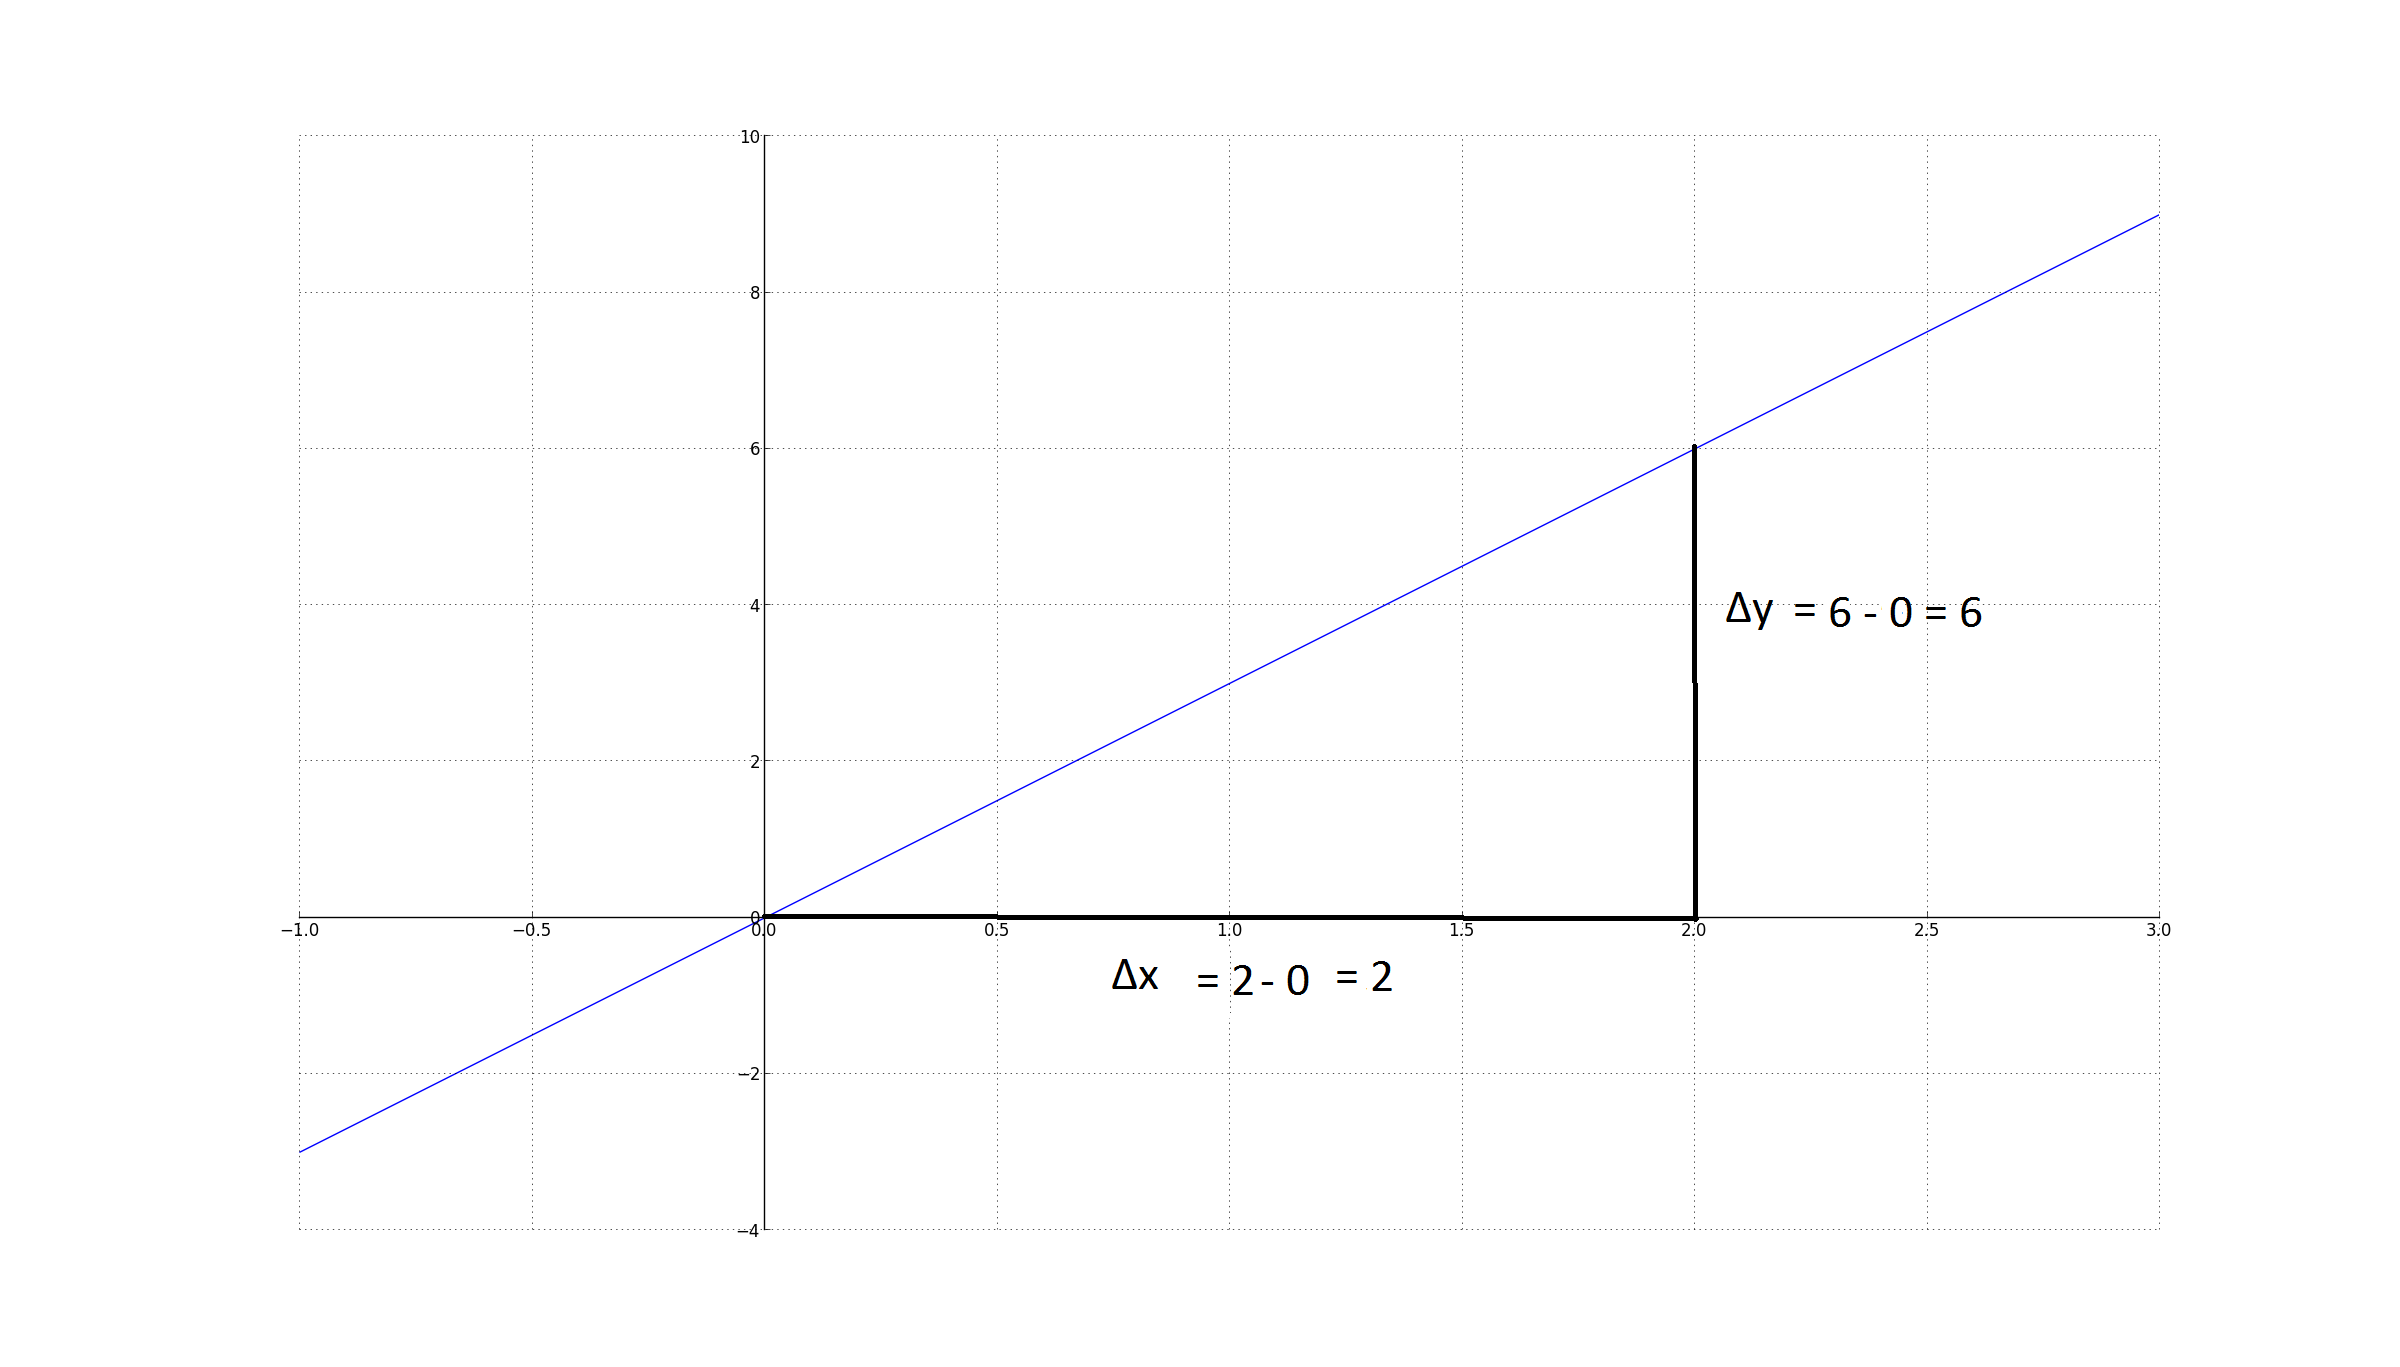
\includegraphics[scale = 0.3]{figures/stigningstalleksempelet.png}
\end{figure}

\subsection*{Konstantledd}

\subsection*{Linear funksjon}
I disse oppgavene  skal vi skrive likninger til linearefunksjoner. Husk at en linje beskrives med linkninger i formen $y=ax+b$ der $a$ er stigningstallet og $b$ er y verdien ved krysnings punkt.

\textbf{Oppgave 1.a}

Skriv likning til en linja som har stigningstallet $4$ og som krysser y aksen på $1$

\textbf{svar}  
$y=4x+1$
\textbf{Hint 1}
Husk at likningen til en linje har formen $y=ax+b$ der $a$ er stigningstallet og $b$ er y verdien ved krysnings punkt.
\textbf{Hint 2}
I dette tilfellet $a=4$ og $b=1$

\textbf{Oppgave 1.b} Hvilken graf tilhører denne funksjon? 
\newline
{\color{Maroon}Det skal vises følgende funksjoner:
$y=4x+1$
\newline
$y=4x+5$
\newline
$y=1x+4$
\newline
$y=5x+3$
\newline
}
\newline\newline

Skriv likning til en linja som har stigningstallet $-2$ og som krysser y aksen på $3$

\textbf{svar}  
$y=4x+1$
\textbf{Hint 1}
Husk at likningen til en linje har formen $y=ax+b$ der $a$ er stigningstallet og $b$ er y verdien ved krysnings punkt.
\textbf{Hint 2}
I dette tilfellet $a=-2$ og $b=3$

\textbf{Oppgave 1.b} Hvilken graf tilhører denne funksjon? 
\newline
{\color{Maroon}Det skal vises følgende funksjoner:
$y=-2x+3$
\newline
$y=2x+-3$
\newline
$y=-3x+2$
\newline
$y=-3x+3$
\newline
}
\newline\newline


 

\end{document}
